% ============================================================
% CHAPTER 5: RESNET - RESIDUAL NETWORK
% ============================================================
\chapter{Residual Network (ResNet)}

\section{Motivation: The Degradation Problem}

\subsection{The Problem with Training Deep Networks}

\paperref{Section 3.2 - ResNet}

\begin{tcolorbox}[colback=yellow!5!white,colframe=yellow!75!black,title=Paper Quote - Degradation Problem]
\textit{``However, when we stack many layers to create an extremely deep network, we discover that the training accuracy begins to saturate and then drops off quickly. These observations lead to the understanding of what is commonly referred to as the degradation problem.''}
\end{tcolorbox}

\begin{figure}[H]
\centering
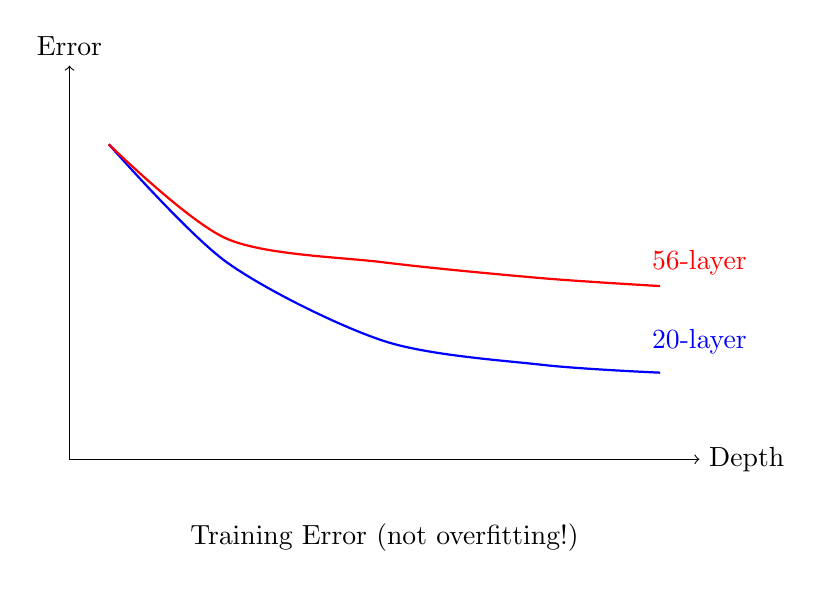
\begin{tikzpicture}
    % Axes
    \draw[->] (0,0) -- (8,0) node[right] {Depth};
    \draw[->] (0,0) -- (0,5) node[above] {Error};
    
    % 20-layer (good)
    \draw[thick, blue] plot[smooth] coordinates {(0.5,4) (2,2.5) (4,1.5) (6,1.2) (7.5,1.1)};
    \node[blue] at (8,1.5) {20-layer};
    
    % 56-layer (bad - degradation)
    \draw[thick, red] plot[smooth] coordinates {(0.5,4) (2,2.8) (4,2.5) (6,2.3) (7.5,2.2)};
    \node[red] at (8,2.5) {56-layer};
    
    \node at (4,-1) {Training Error (not overfitting!)};
\end{tikzpicture}
\caption{Degradation problem: Deeper network has higher error}
\end{figure}

\subsection{Why Does Degradation Occur?}

\begin{tcolorbox}[colback=red!5!white,colframe=red!75!black,title=Key Insight]
Degradation is \textbf{not} due to overfitting (training error also increases).

\textbf{Real cause:}
\begin{itemize}
    \item Optimization difficulty: Hard to find optimal weights
    \item Identity mapping problem: If adding layers, at minimum they should learn identity
    \item But learning identity through non-linear layers is very difficult
\end{itemize}

\textbf{Paradox:} Adding layers \textit{theoretically} cannot reduce performance (worst case: identity), but in practice it does!
\end{tcolorbox}

\section{Residual Learning Framework}

\subsection{Core Idea}

\paperref{Section 3.2 - ResNet}

\begin{tcolorbox}[colback=yellow!5!white,colframe=yellow!75!black,title=Paper Quote - Skip Connections]
\textit{``To solve the degradation problem, ResNet uses an architecture with residual learning framework called skip connections. Instead of hoping each few stacked layers directly fit a desired underlying mapping, skip connections allow the model to bypass certain layers.''}
\end{tcolorbox}

\subsection{Mathematical Formulation}

\textbf{Plain Network:}
\begin{equation}
y = F(x)
\end{equation}

\textbf{Residual Network:}
\begin{equation}
y = F(x) + x
\end{equation}

Where:
\begin{itemize}
    \item $x$: Input to the block
    \item $F(x)$: Residual function (stacked layers)
    \item $y$: Output = residual + identity
\end{itemize}

\begin{figure}[H]
\centering
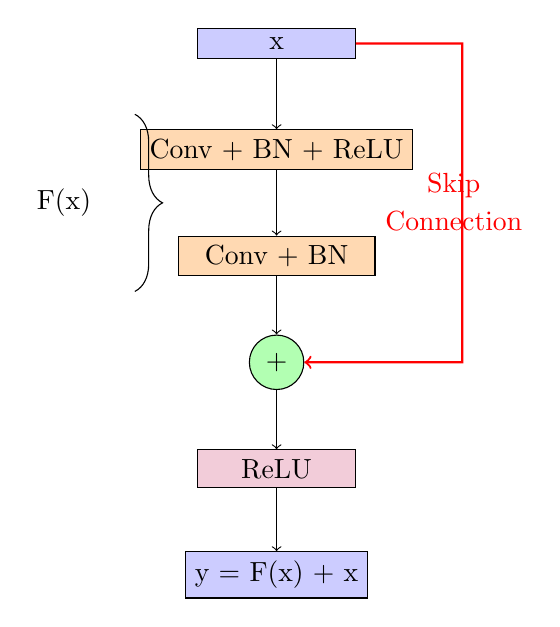
\begin{tikzpicture}[scale=0.9]
    % Input
    \node[draw, fill=blue!20, minimum width=2cm] (input) at (0,0) {x};
    
    % Weight layer 1
    \node[draw, fill=orange!30, minimum width=2.5cm] (w1) at (0,-1.5) {Conv + BN + ReLU};
    
    % Weight layer 2
    \node[draw, fill=orange!30, minimum width=2.5cm] (w2) at (0,-3) {Conv + BN};
    
    % Addition
    \node[draw, circle, fill=green!30] (add) at (0,-4.5) {+};
    
    % ReLU
    \node[draw, fill=purple!20, minimum width=2cm] (relu) at (0,-6) {ReLU};
    
    % Output
    \node[draw, fill=blue!20, minimum width=2cm] (output) at (0,-7.5) {y = F(x) + x};
    
    % Skip connection
    \draw[->] (input) -- (w1);
    \draw[->] (w1) -- (w2);
    \draw[->] (w2) -- (add);
    \draw[->, thick, red] (input.east) -- ++(1.5,0) -- ++(0,-4.5) -- (add.east);
    \node[red] at (2.5,-2) {Skip};
    \node[red] at (2.5,-2.5) {Connection};
    
    \draw[->] (add) -- (relu);
    \draw[->] (relu) -- (output);
    
    % F(x) label
    \draw[decorate, decoration={brace, amplitude=10pt}] (-2,-1) -- (-2,-3.5);
    \node at (-3,-2.25) {F(x)};
\end{tikzpicture}
\caption{Residual Block with Skip Connection}
\end{figure}

\subsection{Why Do Skip Connections Work?}

\begin{tcolorbox}[colback=green!5!white,colframe=green!75!black,title=Benefits of Skip Connections]
\begin{enumerate}
    \item \textbf{Easy to learn identity:}
    \begin{itemize}
        \item If $F(x) = 0$ → $y = x$ (identity)
        \item Learning $F(x) = 0$ is easier than learning complex identity mapping
    \end{itemize}
    
    \item \textbf{Better gradient flow:}
    \begin{itemize}
        \item Gradient has a shortcut through skip connection
        \item Does not vanish through many layers
    \end{itemize}
    
    \item \textbf{Ensemble effect:}
    \begin{itemize}
        \item ResNet can be viewed as an ensemble of many shallow networks
        \item Skip connections create exponential paths
    \end{itemize}
\end{enumerate}
\end{tcolorbox}

\subsection{Gradient Flow Analysis}

\begin{equation}
\frac{\partial \mathcal{L}}{\partial x} = \frac{\partial \mathcal{L}}{\partial y} \cdot \frac{\partial y}{\partial x} = \frac{\partial \mathcal{L}}{\partial y} \cdot \left(1 + \frac{\partial F(x)}{\partial x}\right)
\end{equation}

\begin{tcolorbox}[colback=blue!5!white,colframe=blue!75!black,title=Key Observation]
Gradient always has a ``1'' component from skip connection.

Even when $\frac{\partial F(x)}{\partial x}$ is very small (vanishing), gradient can still flow!
\end{tcolorbox}

\section{ResNet-34 Architecture}

\paperref{Section 3.2 - ResNet}

\subsection{Paper Description}

\begin{tcolorbox}[colback=yellow!5!white,colframe=yellow!75!black,title=Paper Quote - ResNet Architecture]
\textit{``Similar to VGG-19, ResNet comprises multiple residual blocks, each featuring convolutional layers with 3 × 3 filters. A key difference from the VGG-19 is the presence of skip connections. There are 34 weighted layers in this network, and the input image is 224 × 224.''}
\end{tcolorbox}

\subsection{Architecture Details}

\begin{table}[H]
\centering
\caption{ResNet-34 Architecture}
\begin{tabular}{cccc}
\toprule
\textbf{Stage} & \textbf{Output Size} & \textbf{Layers} & \textbf{Blocks} \\
\midrule
conv1 & 112 × 112 & 7×7 conv, 64, stride 2 & - \\
\midrule
conv2\_x & 56 × 56 & 3×3 max pool, stride 2 & 3 \\
 & & $\begin{bmatrix} 3×3, 64 \\ 3×3, 64 \end{bmatrix}$ & \\
\midrule
conv3\_x & 28 × 28 & $\begin{bmatrix} 3×3, 128 \\ 3×3, 128 \end{bmatrix}$ & 4 \\
\midrule
conv4\_x & 14 × 14 & $\begin{bmatrix} 3×3, 256 \\ 3×3, 256 \end{bmatrix}$ & 6 \\
\midrule
conv5\_x & 7 × 7 & $\begin{bmatrix} 3×3, 512 \\ 3×3, 512 \end{bmatrix}$ & 3 \\
\midrule
 & 1 × 1 & Global Avg Pool, FC 15 & - \\
\bottomrule
\end{tabular}
\end{table}

\textbf{Total layers:} $1 + 2 \times (3 + 4 + 6 + 3) + 1 = 34$ weighted layers

\section{Code Implementation}

\coderef{resnet.ipynb}

\subsection{BasicBlock Class}

\begin{lstlisting}[caption={BasicBlock for ResNet-18/34}]
class BasicBlock(nn.Module):
    """
    Basic building block for ResNet-18 and ResNet-34.
    Uses two 3x3 convolutions with skip connection.
    """
    expansion = 1  # Output channels = input channels
    
    def __init__(self, in_channels, out_channels, stride=1, downsample=None):
        super(BasicBlock, self).__init__()
        
        # ===== First conv layer =====
        # Paper: "3x3 convolution"
        self.conv1 = nn.Conv2d(
            in_channels, out_channels,
            kernel_size=3,
            stride=stride,      # stride=2 for downsampling
            padding=1,
            bias=False          # BN handles bias
        )
        self.bn1 = nn.BatchNorm2d(out_channels)
        
        # ===== Second conv layer =====
        self.conv2 = nn.Conv2d(
            out_channels, out_channels,
            kernel_size=3,
            stride=1,
            padding=1,
            bias=False
        )
        self.bn2 = nn.BatchNorm2d(out_channels)
        
        # ===== Skip connection =====
        # If dimensions change, need 1x1 conv to match
        self.downsample = downsample
        self.stride = stride
        
    def forward(self, x):
        identity = x  # Save for skip connection
        
        # Main path: conv -> bn -> relu -> conv -> bn
        out = self.conv1(x)
        out = self.bn1(out)
        out = F.relu(out)
        
        out = self.conv2(out)
        out = self.bn2(out)
        
        # Skip connection (match dimensions if needed)
        if self.downsample is not None:
            identity = self.downsample(x)
        
        # Add skip connection
        out += identity  # y = F(x) + x
        out = F.relu(out)  # Final activation
        
        return out
\end{lstlisting}

\subsection{ResNet Main Class}

\begin{lstlisting}[caption={ResNet-34 main class}]
class ResNet(nn.Module):
    def __init__(self, block, layers, num_classes=15):
        """
        Args:
            block: BasicBlock (for ResNet-18/34) or Bottleneck (for 50/101/152)
            layers: [3, 4, 6, 3] for ResNet-34
            num_classes: 15 for chest x-ray
        """
        super(ResNet, self).__init__()
        self.in_channels = 64
        
        # ===== Initial Convolution =====
        # Paper: "7x7 conv, 64, stride 2"
        self.conv1 = nn.Conv2d(
            3, 64, 
            kernel_size=7, 
            stride=2, 
            padding=3,
            bias=False
        )
        self.bn1 = nn.BatchNorm2d(64)
        self.relu = nn.ReLU(inplace=True)
        
        # Paper: "3x3 max pool, stride 2"
        self.maxpool = nn.MaxPool2d(kernel_size=3, stride=2, padding=1)
        
        # ===== Residual Stages =====
        # layers = [3, 4, 6, 3] for ResNet-34
        self.layer1 = self._make_layer(block, 64, layers[0])       # 3 blocks
        self.layer2 = self._make_layer(block, 128, layers[1], stride=2)  # 4 blocks
        self.layer3 = self._make_layer(block, 256, layers[2], stride=2)  # 6 blocks
        self.layer4 = self._make_layer(block, 512, layers[3], stride=2)  # 3 blocks
        
        # ===== Global Average Pooling =====
        self.avgpool = nn.AdaptiveAvgPool2d((1, 1))
        
        # ===== Classification Head =====
        self.fc = nn.Linear(512 * block.expansion, num_classes)
        
        # ===== Weight Initialization =====
        self._initialize_weights()
        
    def _make_layer(self, block, out_channels, blocks, stride=1):
        """Create a stage with multiple residual blocks."""
        downsample = None
        
        # If spatial size or channels change, need projection
        if stride != 1 or self.in_channels != out_channels * block.expansion:
            downsample = nn.Sequential(
                nn.Conv2d(
                    self.in_channels,
                    out_channels * block.expansion,
                    kernel_size=1,
                    stride=stride,
                    bias=False
                ),
                nn.BatchNorm2d(out_channels * block.expansion)
            )
        
        layers = []
        # First block may have stride > 1 (downsampling)
        layers.append(block(self.in_channels, out_channels, stride, downsample))
        self.in_channels = out_channels * block.expansion
        
        # Remaining blocks have stride = 1
        for _ in range(1, blocks):
            layers.append(block(self.in_channels, out_channels))
        
        return nn.Sequential(*layers)
    
    def _initialize_weights(self):
        """Kaiming initialization for conv layers."""
        for m in self.modules():
            if isinstance(m, nn.Conv2d):
                nn.init.kaiming_normal_(
                    m.weight, mode='fan_out', nonlinearity='relu'
                )
            elif isinstance(m, nn.BatchNorm2d):
                nn.init.constant_(m.weight, 1)
                nn.init.constant_(m.bias, 0)
    
    def forward(self, x):
        # Initial: 224x224x3 -> 112x112x64 -> 56x56x64
        x = self.conv1(x)      # 224 -> 112
        x = self.bn1(x)
        x = self.relu(x)
        x = self.maxpool(x)    # 112 -> 56
        
        # Residual stages
        x = self.layer1(x)     # 56x56x64
        x = self.layer2(x)     # 28x28x128
        x = self.layer3(x)     # 14x14x256
        x = self.layer4(x)     # 7x7x512
        
        # Global average pooling + FC
        x = self.avgpool(x)    # 1x1x512
        x = torch.flatten(x, 1)
        x = self.fc(x)         # 15 classes
        
        return x
\end{lstlisting}

\subsection{Model Instantiation}

\begin{lstlisting}[caption={Creating ResNet-34 instance}]
def resnet34(num_classes=15):
    """Create ResNet-34 model."""
    return ResNet(
        block=BasicBlock,
        layers=[3, 4, 6, 3],  # ResNet-34 configuration
        num_classes=num_classes
    )

# Usage
model = resnet34(num_classes=15)
\end{lstlisting}

\section{Detailed Mapping: Paper → Code}

\begin{table}[H]
\centering
\caption{ResNet-34: Paper → Code Mapping}
\begin{tabular}{p{4cm}p{5cm}p{4cm}}
\toprule
\textbf{Paper Description} & \textbf{PyTorch Code} & \textbf{Output} \\
\midrule
``34 weighted layers'' & \texttt{layers=[3,4,6,3]} → $2 \times 16 + 2 = 34$ & - \\
``7×7 conv, stride 2'' & \texttt{nn.Conv2d(3,64,7,stride=2,padding=3)} & 112×112×64 \\
``3×3 max pool'' & \texttt{nn.MaxPool2d(3,stride=2,padding=1)} & 56×56×64 \\
``skip connections'' & \texttt{out += identity} & - \\
``3×3 filters'' & \texttt{kernel\_size=3} in BasicBlock & - \\
\bottomrule
\end{tabular}
\end{table}

\section{Batch Normalization}

\subsection{Formula}

\begin{equation}
\hat{x}_i = \frac{x_i - \mu_B}{\sqrt{\sigma_B^2 + \epsilon}}
\end{equation}
\begin{equation}
y_i = \gamma \hat{x}_i + \beta
\end{equation}

Where:
\begin{itemize}
    \item $\mu_B, \sigma_B^2$: Mean and variance of mini-batch
    \item $\gamma, \beta$: Learnable scale and shift
    \item $\epsilon$: Small constant for numerical stability
\end{itemize}

\subsection{Why is BatchNorm Important for ResNet?}

\begin{tcolorbox}[colback=blue!5!white,colframe=blue!75!black,title=BatchNorm Benefits]
\begin{enumerate}
    \item \textbf{Internal Covariate Shift:} Normalizing activations helps training stability
    \item \textbf{Higher Learning Rate:} Can use higher LR
    \item \textbf{Regularization Effect:} Reduces overfitting (slightly)
    \item \textbf{ResNet Specific:} BN before skip connection helps gradient flow better
\end{enumerate}
\end{tcolorbox}

\section{Global Average Pooling vs Flatten}

\subsection{Comparison}

\begin{table}[H]
\centering
\caption{Global Average Pooling vs Flatten}
\begin{tabular}{lcc}
\toprule
\textbf{Aspect} & \textbf{Flatten (CNN)} & \textbf{GAP (ResNet)} \\
\midrule
Output size & $H \times W \times C$ & $C$ \\
Parameters in FC & Very large & Small \\
Overfitting risk & High & Low \\
Spatial info & Preserved & Lost (averaged) \\
Translation invariance & No & Yes \\
\bottomrule
\end{tabular}
\end{table}

\subsection{Concrete Example}

\begin{lstlisting}[caption={GAP vs Flatten comparison}]
# After conv layers: feature map is 7x7x512

# Option 1: Flatten (like CNN)
flatten_output = 7 * 7 * 512  # = 25,088
fc_params = 25088 * 15 + 15   # = 376,335 parameters

# Option 2: Global Average Pooling (like ResNet)
gap_output = 512  # Average over 7x7 spatial dims
fc_params = 512 * 15 + 15     # = 7,695 parameters

# GAP reduces 98% parameters in FC layer!
\end{lstlisting}

\section{Parameter Count Analysis}

\begin{table}[H]
\centering
\caption{ResNet-34 Parameter Breakdown}
\begin{tabular}{lcrr}
\toprule
\textbf{Stage} & \textbf{Blocks} & \textbf{Channels} & \textbf{Params} \\
\midrule
conv1 & 1 & 3 → 64 & 9,408 \\
layer1 & 3 & 64 → 64 & 221,184 \\
layer2 & 4 & 64 → 128 & 1,114,624 \\
layer3 & 6 & 128 → 256 & 6,818,304 \\
layer4 & 3 & 256 → 512 & 13,631,488 \\
FC & 1 & 512 → 15 & 7,695 \\
\midrule
\textbf{Total} & & & \textbf{21,802,703} \\
\bottomrule
\end{tabular}
\end{table}

\textbf{Comparison:} ResNet-34 has \textbf{21M params} vs CNN's \textbf{102M params}, but is deeper (34 layers vs 4 layers) and more effective!

\section{Results Analysis}

\paperref{Section 5 - Experiments}

\subsection{Paper Results}

\begin{tcolorbox}[colback=yellow!5!white,colframe=yellow!75!black,title=Paper Results - ResNet]
\begin{itemize}
    \item \textbf{Training Accuracy:} 93\%
    \item \textbf{Validation AUC:} 0.86
    \item \textbf{Test AUC:} 0.86
\end{itemize}
\end{tcolorbox}

\subsection{Comparison with CNN}

\begin{table}[H]
\centering
\caption{CNN vs ResNet Performance}
\begin{tabular}{lcc}
\toprule
\textbf{Metric} & \textbf{CNN} & \textbf{ResNet-34} \\
\midrule
Training Accuracy & 91\% & 93\% (+2\%) \\
Test AUC & 0.82 & 0.86 (+0.04) \\
Parameters & 102M & 21M \\
Depth & 4 layers & 34 layers \\
\bottomrule
\end{tabular}
\end{table}

\subsection{Why is ResNet Better?}

\begin{tcolorbox}[colback=green!5!white,colframe=green!75!black,title=Analysis: ResNet Advantages]
\begin{enumerate}
    \item \textbf{Deeper Feature Hierarchy:}
    \begin{itemize}
        \item 34 layers vs 4 layers
        \item Can learn complex hierarchical features
        \item X-ray patterns have many levels of abstraction
    \end{itemize}
    
    \item \textbf{Better Gradient Flow:}
    \begin{itemize}
        \item Skip connections allow direct gradient flow
        \item More stable training
    \end{itemize}
    
    \item \textbf{Efficient Parameter Usage:}
    \begin{itemize}
        \item GAP instead of flatten
        \item Fewer parameters but more expressive
    \end{itemize}
    
    \item \textbf{Better Regularization:}
    \begin{itemize}
        \item Batch Normalization in every block
        \item Weight decay is more effective
    \end{itemize}
\end{enumerate}
\end{tcolorbox}
